\section{GraphRA6 Klassenreferenz}
\label{classGraphRA6}\index{GraphRA6@{GraphRA6}}
Klassendiagramm für GraphRA6::\begin{figure}[H]
\begin{center}
\leavevmode
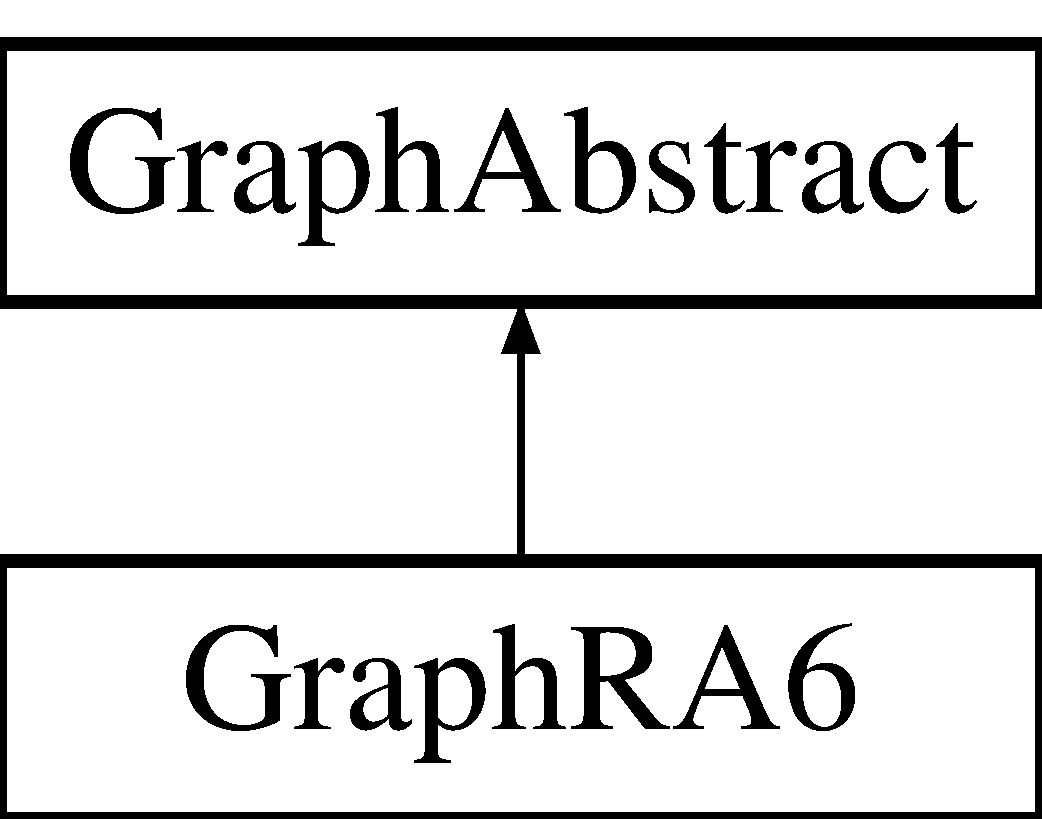
\includegraphics[height=2cm]{classGraphRA6}
\end{center}
\end{figure}
\subsection*{Öffentliche Methoden}
\begin{CompactItemize}
\item 
{\bf GraphRA6} (\$graphId)
\end{CompactItemize}


\subsection{Ausführliche Beschreibung}


Definiert in Zeile 10 der Datei class.GraphRA6.php.

\subsection{Dokumentation der Elementfunktionen}
\index{GraphRA6@{GraphRA6}!GraphRA6@{GraphRA6}}
\index{GraphRA6@{GraphRA6}!GraphRA6@{GraphRA6}}
\subsubsection{\setlength{\rightskip}{0pt plus 5cm}GraphRA6.GraphRA6 (\$ {\em graphId})}\label{classGraphRA6_da71fd7949b0b4401b50df2a46dad845}




Definiert in Zeile 12 der Datei class.GraphRA6.php.

Die Dokumentation für diese Klasse wurde erzeugt aufgrund der Datei:\begin{CompactItemize}
\item 
{\bf class.GraphRA6.php}\end{CompactItemize}
